
\subsection{Calorimeter Calibration}
In order to have a constant L0 rate the calorimeter gain should not
change with time.
The variation of the gain can be estimated by the variation of the
relative occupancy. The occupancy for a cell is defined as the fraction of events in which
the ADC output is above a  threshold. The ratio of the occupancies with respect to a
reference sample is proportional to the changes in gain.
A relative calibration is performed online on a single node for each fill using this occupancy
method and when needed the high voltage is changed accordingly. 

An absolute calibration can be obtained with the $\pi^0$ method: the
reconstructed $\pi^0$ mass can be determined for each cell by fitting di-photon
mass distributions where one of the photon has the cell as the seed. The
calibration coefficients can be tuned to constrain the reconstructed $\pi^0$ mass
 to the nominal one. This fine calibration requires an iterative procedure and
 it is run on the HLT farm similarly to the tracking or RICH mirror alignment. 
This second method takes several hours to run and will be
performed a few times per year i.e. during technical stops.

\subsubsection{Calibration with Relative Occupancy and LEDs}

\begin{figure}[h]
\begin{minipage}{0.5\columnwidth}
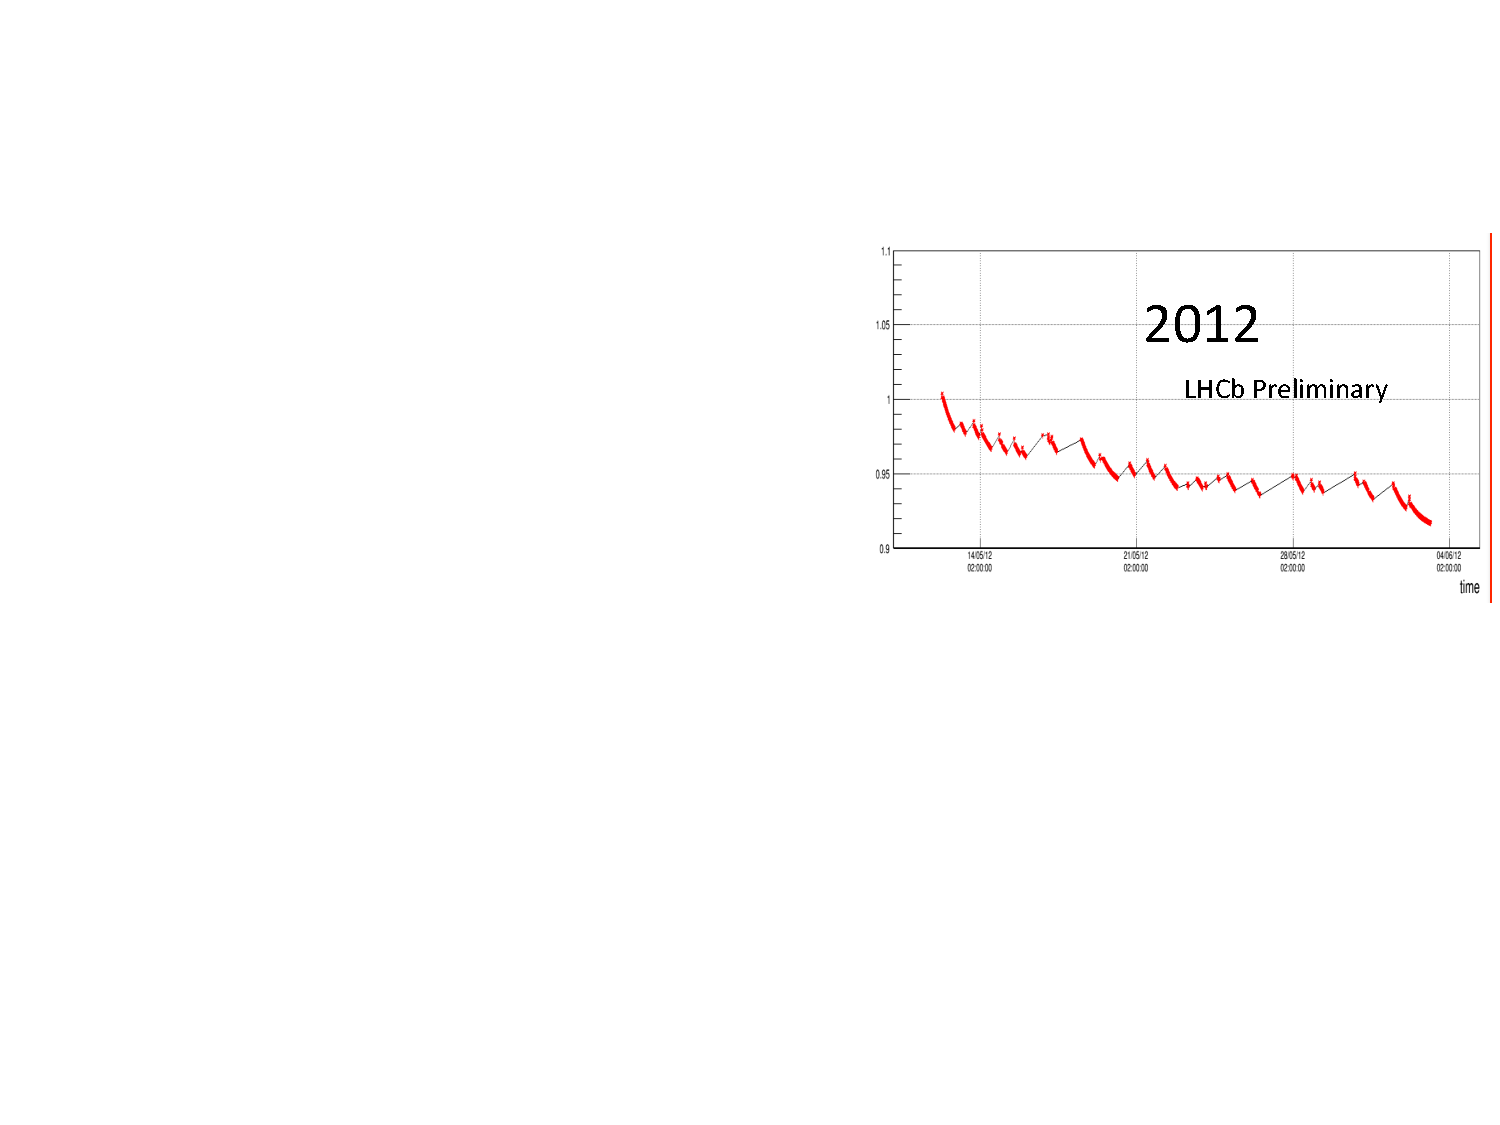
\includegraphics[width=\columnwidth]{../figures/CaloStability2012}
\end{minipage}\hspace{2pc}%
\begin{minipage}{0.5\columnwidth}
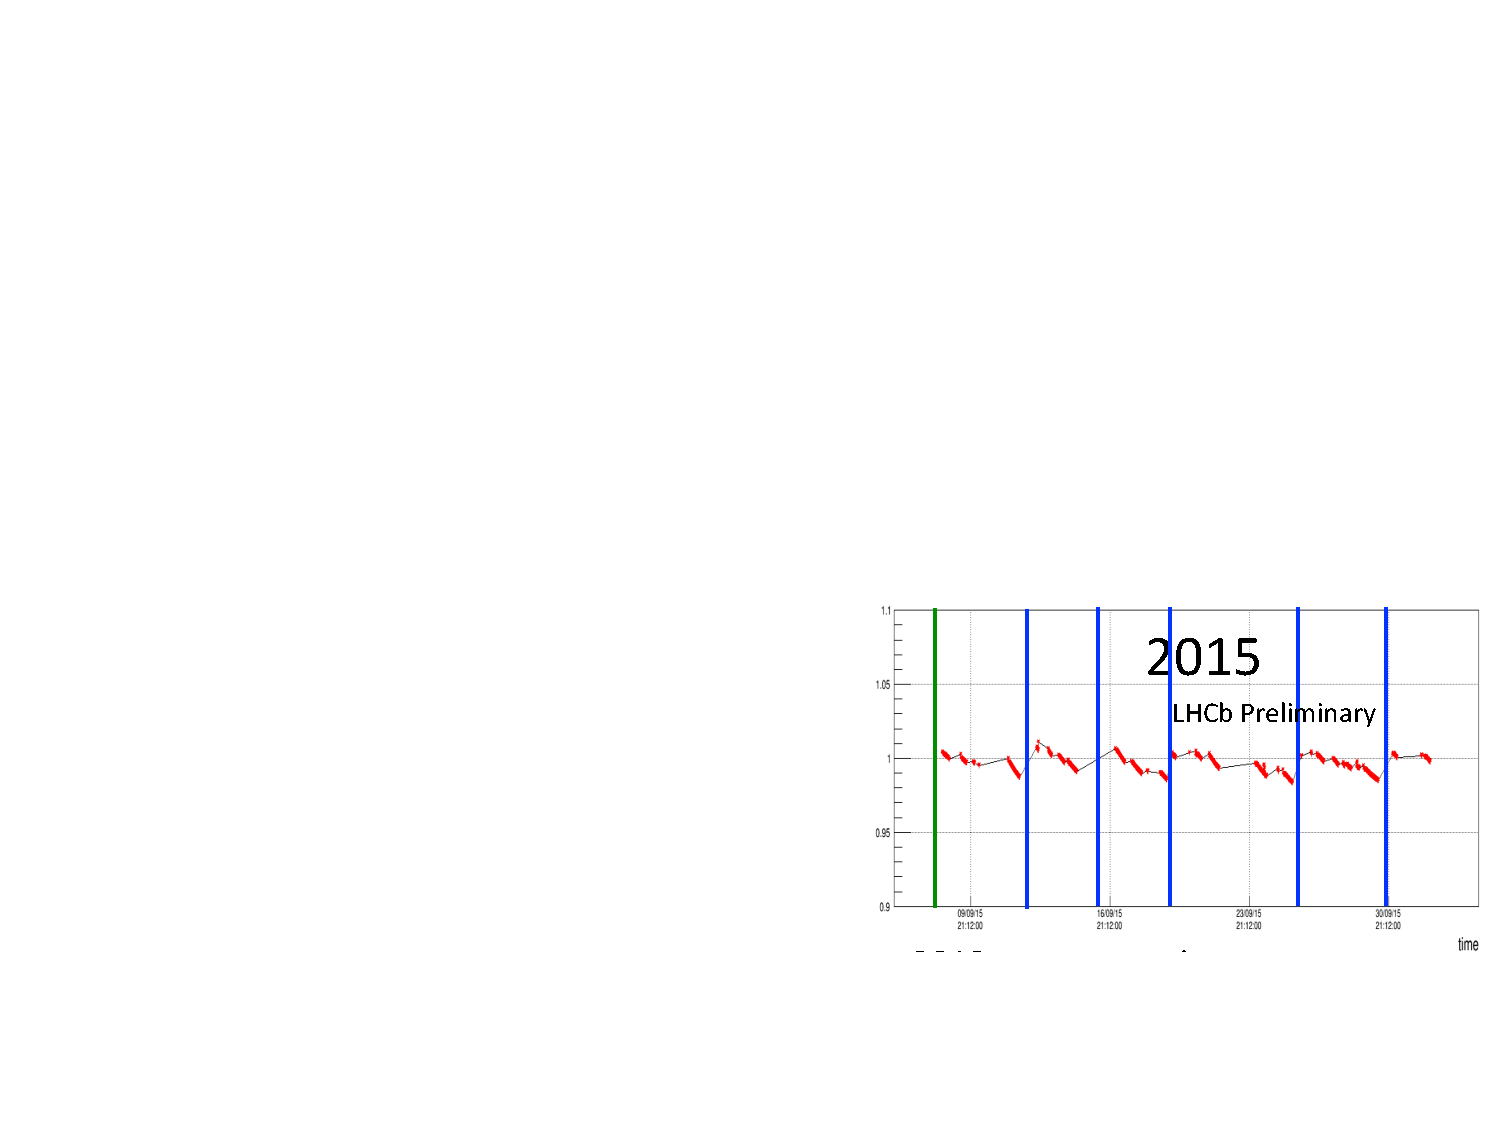
\includegraphics[width=\columnwidth]{../figures/CaloStability2015}
\end{minipage} 
\caption{\label{fig:CaloStability} Stability of calorimeter calibration. Caption to be written, 1st draft for the plot}
\end{figure}

\subsubsection{Absolute Calibration for HCAL with Cs source}


\subsubsection{Absolute Calibration for ECAL with \texorpdfstring{\piz}{pi0}}

\begin{figure}[h]
  \centering
  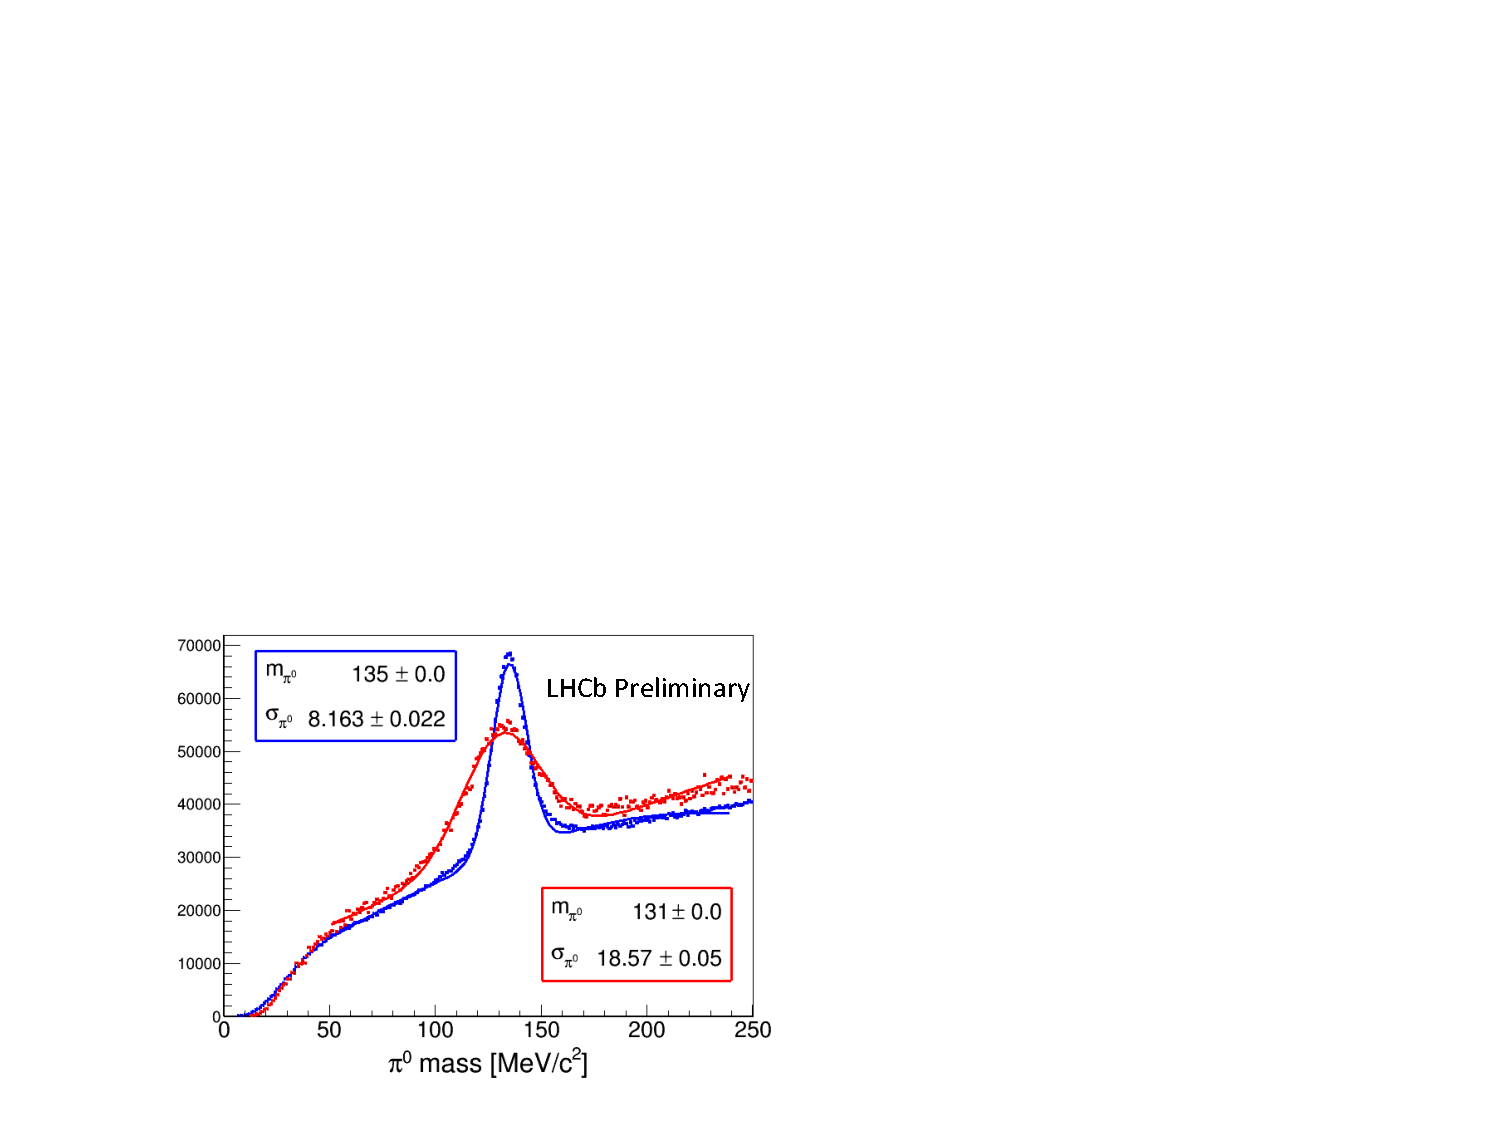
\includegraphics[width=8cm]{../figures/CaloPi0Calibration2015}
  \caption{ Stability of calorimeter calibration. Caption to be written, 1st draft for the plot}
  \label{fig:Calo_Pi0calib}
\end{figure}





